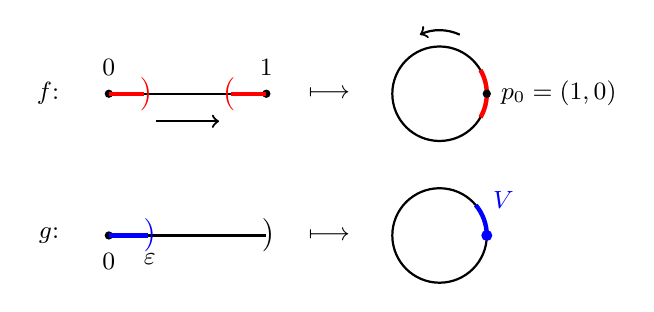
\begin{tikzpicture}[line width=0.8pt, every node/.style={font=\small}]
  % f : [0,1] -> S^1
  \node[anchor=east] at (-0.5,0) {$f$:};
  \draw (0,0) -- (2,0);
  \fill (0,0) circle (1.5pt) (2,0) circle (1.5pt);
  \node[above] at (0,0.1) {$0$};
  \node[above] at (2,0.1) {$1$};
  \draw[red, line width=1.6pt] (0,0) -- (0.45,0);
  \node[red] at (0.47,0) {\large )};
  \draw[red, line width=1.6pt] (1.55,0) -- (2,0);
  \node[red] at (1.53,0) {\large (};
  \draw[->] (0.6,-0.35) -- (1.4,-0.35);
  \node at (2.8,0) {$\longmapsto$};
  \draw (4.2,0) circle (0.6);
  \draw[red, line width=1.6pt] (4.2,0) ++(-30:0.6) arc[start angle=-30, end angle=30, radius=0.6];
  \fill (4.8,0) circle (1.5pt);
  \node[right] at (4.85,0) {$p_0=(1,0)$};
  \draw[<-] (3.95,0.75) arc[start angle=115, end angle=65, radius=0.6];
  % g = f restricted to [0,1)
  \node[anchor=east] at (-0.5,-1.8) {$g$:};
  \draw (0,-1.8) -- (2,-1.8);
  \node at (2.02,-1.8) {\large )};
  \fill (0,-1.8) circle (1.5pt);
  \node[below] at (0,-1.9) {$0$};
  \draw[blue, line width=1.6pt] (0,-1.8) -- (0.5,-1.8);
  \node[blue] at (0.52,-1.8) {\large )};
  \node[below] at (0.52,-1.9) {$\varepsilon$};
  \node at (2.8,-1.8) {$\longmapsto$};
  \draw (4.2,-1.8) circle (0.6);
  \draw[blue, line width=1.6pt] (4.2,-1.8) ++(0:0.6) arc[start angle=0, end angle=40, radius=0.6];
  \fill[blue] (4.8,-1.8) circle (2pt);
  \node[blue, right] at (4.75,-1.35) {$V$};
\end{tikzpicture}
